% Para compilar, use:
% pdflatex -shell-escape melissa_blusol13.tex
%%%%%%%%%%%%%%%%%%%%%%%%%%%%%%%%%%%%%%%%%%%%%%%%%%%%%%%%%%%%%%%%%%%%%%%%%%%%%%%%%%%%%%%%%
% PREAMBULO
%%%%%%%%%%%%%%%%%%%%%%%%%%%%%%%%%%%%%%%%%%%%%%%%%%%%%%%%%%%%%%%%%%%%%%%%%%%%%%%%%%%%%%%%%
\documentclass{beamer}
\usetheme{default}
\setbeamercovered{transparent}
\usecolortheme{seagull}
\usefonttheme{structurebold}
% Cores
\definecolor{practice}{rgb}{0.02,0.1,0.45}
\definecolor{europeanalonis}{rgb}{0.49,0.19,1}
\definecolor{azulin}{rgb}{0.24,0.43,1}
\definecolor{skythegirl}{rgb}{0.25,0.59,1}
\definecolor{jeeziecreezie}{rgb}{0.55,0.98,1}
\definecolor{pinegreen}{rgb}{0.02,0.58,0}
% Opcoes do beamer
\setbeamertemplate{footline}
{%
   
\includegraphics[trim=0mm 7mm 0mm 0mm,clip]{img/textura_flowers.png}
}
\usenavigationsymbolstemplate{}
\setbeamercolor{normal text}{fg=practice}
\setbeamercolor{frametitle}{fg=azulin}
\setbeamercolor{structure}{fg=practice}
\setbeamercolor{block body}{bg=azulin,fg=jeeziecreezie!20}
\setbeamercolor{alerted text}{fg=europeanalonis}

% Pacotes adicionais
\usepackage[portuguese]{babel}
\usepackage[utf8]{inputenc} % Para usar acentos
\usepackage[T1]{fontenc} % Carrega algumas opções de fontes especiais
\usepackage{minted} % Para mostrar código com realce de sintaxe
                    % Para usar o pacote minted você deve instalar o 
                    % pygments (biblioteca em Python)
                    % Na maioria das distros linux, isso se faz com o comando
                    % # pip install pygments
\usepackage{tikz} % Para fazer gráficos
\usetikzlibrary{shapes,arrows} % Biblioteca de formas do TikZ
\usetikzlibrary{decorations.text}
\let\Tiny=\tiny % Elimina alguns avisos de compilação do beamer

% Novo macro para exibir palavras chave em cores
\newcommand{\kw}[1]{\textbackslash {\color{europeanalonis}#1}}

% Informacoes
\title{\textcolor{europeanalonis}{Automatizando a criação de PDFs com \LaTeX+Python}} \author[M. Weber Mendonça]
{\hspace{-0.3cm}Melissa Weber Mendonça\inst{1}}
\institute[UFSC]{\inst{1} Universidade Federal de Santa Catarina}
\date{Warm up - SciPy-LA 2016}

\logo{\includegraphics[height=1.5cm]{/home/melissa/Dropbox/Documentos/latex/brasao_UFSC.png}} % Logo para todos os slides. Não incluido nos arquivos distribuidos.
%%%%%%%%%%%%%%%%%%%%%%%%%%%%%%%%%%%%%%%%%%%%%%%%%%%%%%%%%%%%%%%%%%%%%%%%%%%%%%%%%%%%%%%%%

\begin{document}
\begin{frame}
  \titlepage
\end{frame}
\begin{frame}
   \frametitle{O que é \LaTeX? \small{(e por que está escrito desse jeito??)}}
   O \LaTeX\ é um sistema de composição tipográfica de alta qualidade, e é o padrão na comunicação e publicação de documentos científicos.
   \begin{columns}
      \column{5cm}
      \begin{center}
         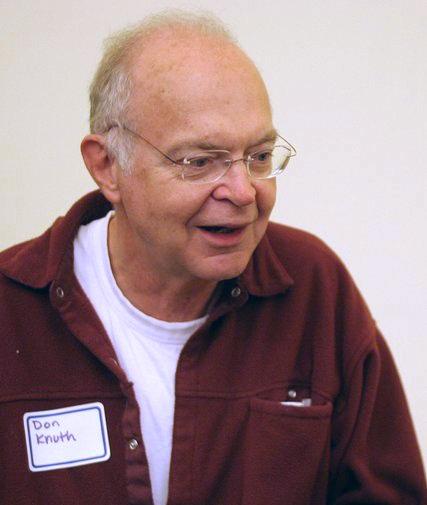
\includegraphics[width=4.7cm]{img/knuth.jpg}\\
         Donald Knuth
      \end{center}
      \column{5cm}
      \begin{center}
         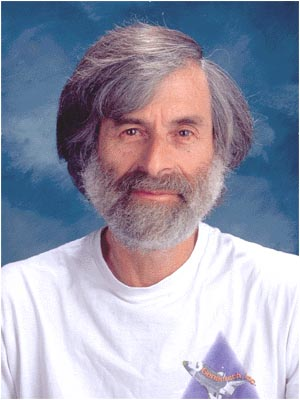
\includegraphics[width=4.2cm]{img/lamport.jpg}\\
         Leslie Lamport
      \end{center}
   \end{columns}
\end{frame}
%%%%%%%%%%%%%%%%%%%%%%%%%%%%%%%%%%%%%%%%%%%%%%%%%%%%%%%%%%%%%%%%%%%%%%%%%%%%%%%%%%%%%%%%%%%%%%%%%%%%%%%
\begin{frame}
   \frametitle{Boa notícia!}
   \begin{center}
      \begin{minipage}{5cm}
        \begin{beamercolorbox}[sep=1em,wd=5cm]{block body}
            \begin{center}
               \LaTeX\ é software livre!
            \end{center}
        \end{beamercolorbox}
      \end{minipage}
      \begin{minipage}{5cm}
         \begin{center}
            
\includegraphics[width=4cm]{img/saintignuciuscopia.jpg}
         \end{center}
      \end{minipage}
   \end{center}
\end{frame}
%%%%%%%%%%%%%%%%%%%%%%%%%%%%%%%%%%%%%%%%%%%%%%%%%%%%%%%%%%%%%%%%%%%%%%%%%%%%%%%%%%%%%%%%%%%%%%%%%%%%%%%
\begin{frame}
   \frametitle{Mas por que usar isso? Não é mais fácil usar o *Office?}
   \begin{center}
         \fbox{
            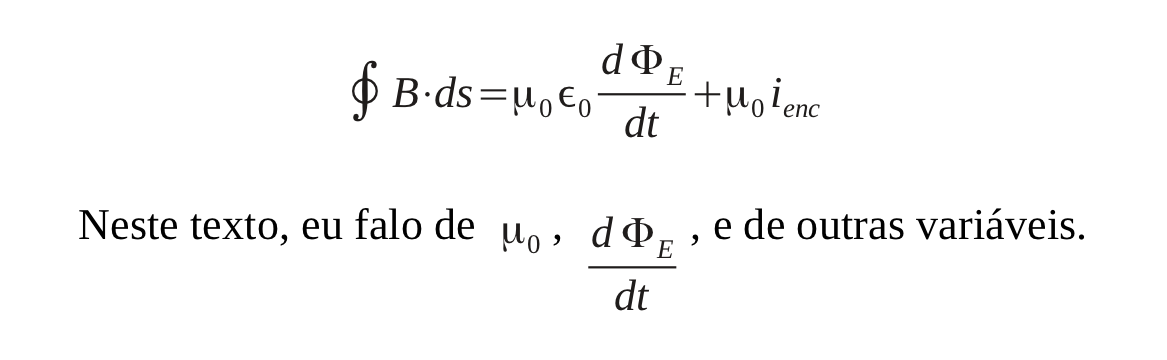
\includegraphics[width=9.25cm]{img/exemplo_libreoffice.png}
            }
      \noindent\framebox[9.6cm]{\parbox{9.25cm}{
            $$\oint B\cdot ds=\mu_0 \epsilon_0 \frac{d\Phi_E}{dt} + \mu_0 i_{enc}$$
            \begin{center}
               Neste texto, eu falo de $\mu_0$, $\displaystyle \frac{d\Phi_E}{dt}$, e de outras coisas.
            \end{center}
         }}
%          }
   \end{center}
\end{frame}
%%%%%%%%%%%%%%%%%%%%%%%%%%%%%%%%%%%%%%%%%%%%%%%%%%%%%%%%%%%%%%%%%%%%%%%%%%%%%%%%%%%%%%%%%%%%%%%%%%%%%%%
\begin{frame}[fragile]
   \frametitle{Código do exemplo anterior}
   \begin{center}
   \noindent\framebox[9.25cm]{\parbox{9.25cm}{
            $$\oint B\cdot ds=\mu_0 \epsilon_0 \frac{d\Phi_E}{dt} + \mu_0 i_{enc}$$
            \begin{center}
               Neste texto, eu falo de $\mu_0$, $\displaystyle \frac{d\Phi_E}{dt}$, e de outras coisas.
            \end{center}
         }}
   \end{center}
   \footnotesize{
   {\tt{
   \$\$\kw{oint} B\kw{cdot} ds = 
      \kw{mu}$\_$0 \kw{epsilon}$\_$0 \kw{frac}\{d\kw{Phi}$\_$E\}\{dt\} + \kw{mu}$\_$0 i$\_$\{enc\}\$\$

   \kw{begin}\{center\}

      Neste texto, eu falo de \$\kw{mu}$\_$0\$, \$\kw{dfrac}\{d\kw{Phi}$\_$E\}\{dt\}\$, 
      e de outras coisas.

   \kw{end}\{center\}
   }}}
\end{frame}
%%%%%%%%%%%%%%%%%%%%%%%%%%%%%%%%%%%%%%%%%%%%%%%%%%%%%%%%%%%%%%%%%%%%%%%%%%%%%%%%%%%%%%%%%%%%%%%%%%%%%%%
\begin{frame}
   \frametitle{Procedimento padrão}
   \begin{columns}
      \column{6cm}
      \begin{itemize}
         \item Escrever código no editor e salvar num arquivo com extensão {\tt{.tex}}
         \uncover<2->{\item Compilar: \\{\tt{pdflatex arquivo.tex}}}
         \uncover<3->{\item Visualizar PDF}
      \end{itemize}
      \column{4cm}
      \begin{tikzpicture}[node distance=2cm, overlay]
         \node (editor) at (1.5,1.5) {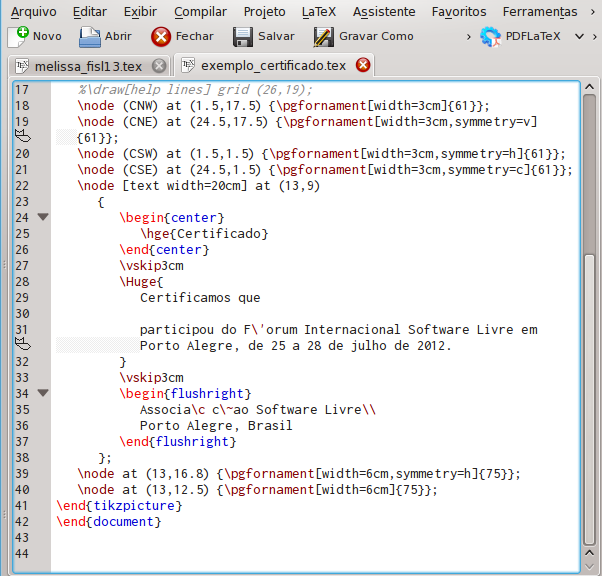
\includegraphics[width=2cm]{img/editor.png}};
         \node [below of=editor] (dummy) {};
         \node<2-> [right of=dummy] (terminal) {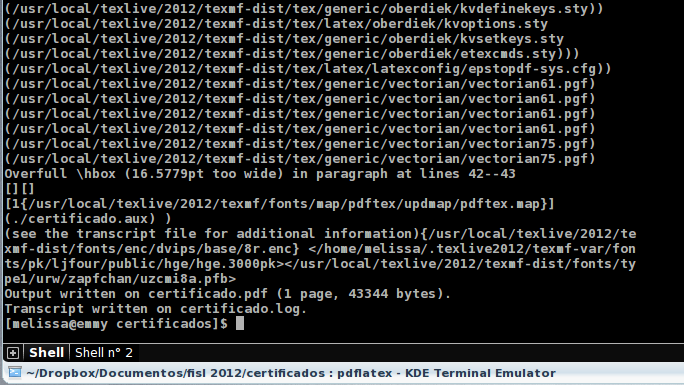
\includegraphics[width=2cm]{img/terminal.png}};
         \node<3-> [below of=dummy] (pdf) {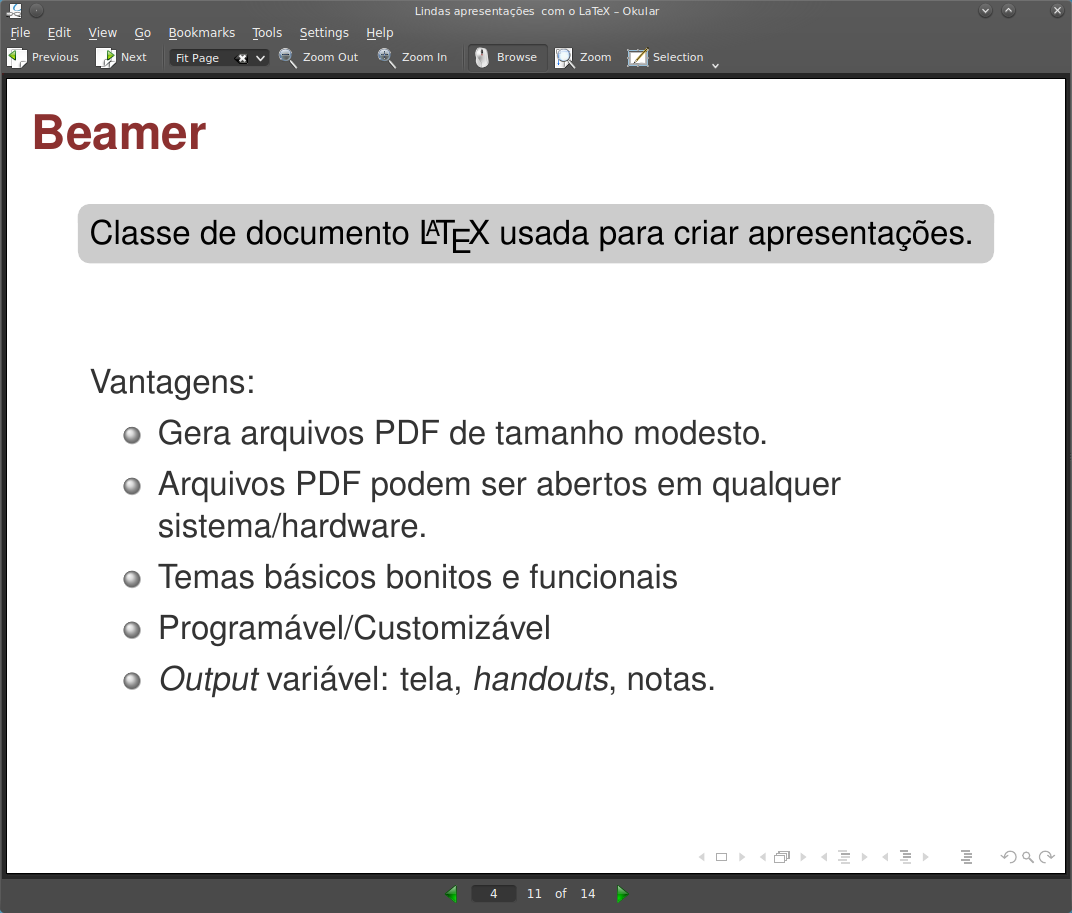
\includegraphics[width=2.5cm]{img/output.png}};
         \path<2->[->] (editor.east) edge [bend left] (terminal.north);
         \path<3->[->] (terminal.south) edge [bend left] (pdf.east);
      \end{tikzpicture}
   \end{columns}
\end{frame}
% %%%%%%%%%%%%%%%%%%%%%%%%%%%%%%%%%%%%%%%%%%%%%%%%%%%%%%%%%%%%%%%%%%%%%%%%%%%%%%%%%%%%%%%%%%%%%%%%%%%%%%%
\begin{frame}
   \frametitle{Estrutura básica de um documento}
   \begin{minipage}{0.2\textwidth}
         \begin{tikzpicture}[overlay,scale=0.5]
            % Para ajudar a fazer os gráficos
            %\draw[step=0.5,black,thin,xshift=0.5cm,yshift=0.5cm] (0,-7) grid (4.5,7);
            \draw<3>[very thick, europeanalonis] (4.5,6.5) to (4.15,6.5);
            \draw<3>[very thick, europeanalonis] (4.2,6.5) to (4.2,2.95);
            \draw<3>[very thick, europeanalonis] (4.5,3.0) to (4.2,3.0);
            \node<3>[europeanalonis] at (2,4.9) {Preâmbulo};
            % 
            \draw<6>[very thick, europeanalonis] (4.5,1.8) to (4.15,1.8);
            \draw<6>[very thick, europeanalonis] (4.2,1.8) to (4.2,-0.8);
            \draw<6>[very thick, europeanalonis] (4.5,-0.75) to (4.2,-0.75);
            \node<6>[europeanalonis] at (2,0.5) {Conteúdo};
         \end{tikzpicture}
      \end{minipage}
      \setbeamercovered{transparent,again covered={\opaqueness<1->{25}}}
      \begin{minipage}{0.75\textwidth}
         \begin{overlayarea}{\textwidth}{0.8\textheight}
            \uncover<1-3,7>{\tt{\kw{documentclass}}\{article\}\\}
            \uncover<2-3,7>{\tt{\kw{title}\{Titulo\}\\
                  \kw{author}\{Seu nome\}\\
                  \kw{date}\{Hoje\}}\\}
              \uncover<4->{\tt{\kw{begin}\{document\}}\\}
              \uncover<5->{\tt{\kw{maketitle}}\\}
              \uncover<6->{Seu texto vai aqui.\\
                \tt{\$\$x = \kw{frac}\{-b \kw{pm} \kw{sqrt}\{b\^{}2-4ac\}\}\{2a\}\$\$}}
              \uncover<4->{\tt{\kw{end}\{document\}}}
         \end{overlayarea}
      \end{minipage}
\end{frame}

% %%%%%%%%%%%%%%%%%%%%%%%%%%%%%%%%%%%%%%%%%%%%%%%%%%%%%%%%%%%%%%%%%%%%%%%%%%%%%%%%%%%%%%%%%%%%%%%%%%%%%%%
\begin{frame}
   \frametitle{Classes de documento}
   \begin{itemize}
      \item \href{exemplo_carta.pdf}{Cartas}
      \item Artigos/Relatórios
      \item \href{beameruserguide.pdf}{Livros}
      \item Apresentações
      \item Estilo ABNT ({\tt{abntex}})
      % Créditos de ornament.pdf para http://altermundus.com/pages/tkz/ornament/index.html
      \item \href{ornament.pdf}{Poesia}
      % Créditos de cv.pdf para http://jblevins.org/projects/cv-template/
      \item \href{cv.pdf}{CV}
      \item \alert{O que você quiser!}
   \end{itemize}
\end{frame}
% %%%%%%%%%%%%%%%%%%%%%%%%%%%%%%%%%%%%%%%%%%%%%%%%%%%%%%%%%%%%%%%%%%%%%%%%%%%%%%%%%%%%%%%%%%%%%%%%%%%%%%%
\begin{frame}
   \frametitle{Fontes}
   \begin{figure}[htbp]
      \includegraphics[viewport=100 550 600 750,width=16cm,clip]%
      {img/fontes.pdf}
      % Fontes usadas: Calligra, Huncial, Sqrcaps, Yfonts, UGQ, Iwona
      % Mais informações no site abaixo.
      % http://www.tug.dk/FontCatalogue/
   \end{figure}
\end{frame}
% %%%%%%%%%%%%%%%%%%%%%%%%%%%%%%%%%%%%%%%%%%%%%%%%%%%%%%%%%%%%%%%%%%%%%%%%%%%%%%%%%%%%%%%%%%%%%%%%%%%%%%%
\begin{frame}[fragile]
   \frametitle{Sintaxe}
   \begin{columns}
   \column{5cm}
      \begin{tabular}{|c|c|c|}
         \hline
         Distros & Gnome & KDE \\\hline
         Ubuntu & X &  \\\hline
         Fedora & X & \\\hline
         Debian & X & \\\hline
         OpenSUSE & & X \\\hline
         Slackware & & X\\
         \hline
      \end{tabular}
   \column{6cm}
   \footnotesize{\tt{%
         \kw{begin}\{tabular\}\{|c|c|c|\}\\
         \qquad \kw{hline}\\
         \qquad Distros \& Gnome \& KDE \kw{}\kw{}\kw{hline}\\
         \qquad Ubuntu \& X \& \kw{}\kw{}\kw{hline}\\
         \qquad Fedora \& X \& \kw{}\kw{}\kw{hline}\\
         \qquad Debian \& X \& \kw{}\kw{}\kw{hline}\\
         \qquad OpenSUSE \& \& X \kw{}\kw{}\kw{hline}\\
         \qquad Slackware \& \& X\kw{}\kw{}\kw{hline}\\
         \kw{end}\{tabular\}
      }}
   \end{columns}
\end{frame}
%%%%%%%%%%%%%%%%%%%%%%%%%%%%%%%%%%%%%%%%%%%%%%%%%%%%%%%%%%%%%%%%%%%%%%%%%%%%%%%%%%%%%%%%%%%%%%%%%%%%%%%
\begin{frame}
   \frametitle{Outras vantagens}
   \begin{itemize}
      \item Numeração automática de seções, capítulos, figuras, tabelas, equações, etc
      \item<2-> Citação automática de itens bibliográficos
      \item<3-> Seleção linguística, incluindo palavras-chave, separação de sílabas, acentos, etc
   \end{itemize}
   \begin{center}
      \href{tudo.tex}{\tt{tudo.tex}}
   \end{center}
\end{frame}
%%%%%%%%%%%%%%%%%%%%%%%%%%%%%%%%%%%%%%%%%%%%%%%%%%%%%%%%%%%%%%%%%%%%%%%%%%%%%%%%%%%%%%%%%%%%%%%%%%%%%%%
\begin{frame}
   \frametitle{Formatação avançada}
   \begin{figure}[htbp]
      \tikz \fill [decorate,decoration={text along path,
        text=teste teste teste teste teste teste teste teste teste teste teste }] plot [smooth, tension=2] coordinates { (0,0) (1,1) (2,-2) (4,1) (5,0)};
   \end{figure}
\end{frame}
%%%%%%%%%%%%%%%%%%%%%%%%%%%%%%%%%%%%%%%%%%%%%%%%%%%%%%%%%%%%%%%%%%%%%%%%%%%%%%%%%%%%%%%%%%%%%%%%%%%%%%%
\begin{frame}
   \frametitle{E...?}
   \only<2->{
     \begin{center}
       \begin{minipage}{6cm}
         \begin{beamercolorbox}[sep=1em,wd=5cm]{block body}
           \begin{center}
             \LaTeX\ é programável!
           \end{center}
         \end{beamercolorbox}
       \end{minipage}
     \end{center}
   }
\end{frame}
%%%%%%%%%%%%%%%%%%%%%%%%%%%%%%%%%%%%%%%%%%%%%%%%%%%%%%%%%%%%%%%%%%%%%%%%%%%%%%%%%%%%%%%%%%%%%%%%%%%%%%%
\begin{frame}[fragile]
  \frametitle{Variáveis}
  {\tt{
     \kw{def}\kw{comando}\{texto\}\\
   
     \kw{newcommand}\{\kw{comando}\}[args]\{def\}
     }}
   \vfill
   \begin{center}
   \href{variaveis.tex}{\tt{variaveis.tex}}
   \end{center}
\end{frame}
\begin{frame}
   \frametitle{Loops: Exemplo}
   \begin{center}
      \begin{minipage}{5cm}
         \begin{center}
            \begin{beamercolorbox}[sep=1em]{block body}
               \begin{center}
                  ingressos.tex
               \end{center}
            \end{beamercolorbox}
         \end{center}
      \end{minipage}
   \end{center}
\end{frame}
% %%%%%%%%%%%%%%%%%%%%%%%%%%%%%%%%%%%%%%%%%%%%%%%%%%%%%%%%%%%%%%%%%%%%%%%%%%%%%%%%%%%%%%%%%%%%%%%%%%%%%%%
\begin{frame}
   \frametitle{E...}
      \begin{center}
         \begin{minipage}{6cm}
         \begin{beamercolorbox}[sep=1em]{block body}
           \begin{center}
             \LaTeX\ pode ser gerado por código!
           \end{center}
         \end{beamercolorbox}
         \end{minipage}
      \end{center}
\end{frame}
% %%%%%%%%%%%%%%%%%%%%%%%%%%%%%%%%%%%%%%%%%%%%%%%%%%%%%%%%%%%%%%%%%%%%%%%%%%%%%%%%%%%%%%%%%%%%%%%%%%%%%%%
\begin{frame}
   \frametitle{Exemplo 1}
   Como gerar um arquivo .pdf com a listagem dos arquivos de um diretório?
   \begin{center}
      \href{diretorio.py}{\tt{diretorio.py}}
   \end{center}
\end{frame}
% %%%%%%%%%%%%%%%%%%%%%%%%%%%%%%%%%%%%%%%%%%%%%%%%%%%%%%%%%%%%%%%%%%%%%%%%%%%%%%%%%%%%%%%%%%%%%%%%%%%%%%%
\begin{frame}
   \frametitle{Exemplo 2}
   Gerar certificados para cada uma das pessoas listadas em um banco de dados SQLite.
   \begin{center}
      \href{certificados.py}{\tt{certificados.py}}
   \end{center}
\end{frame}
%%%%%%%%%%%%%%%%%%%%%%%%%%%%%%%%%%%%%%%%%%%%%%%%%%%%%%%%%%%%%%%%%%%%%%%%%%%%%%%%%%%%%%%%%%%%%%%%%%%%%%%
\begin{frame}
  \frametitle{TikZ}
  \begin{center}
    \begin{minipage}{8cm}
      \begin{beamercolorbox}[sep=1em,wd=8cm]{block body}
        \begin{center}
          "TikZ ist kein Zeichenprogramm" \\("TikZ não é um programa para desenhar")
        \end{center}
      \end{beamercolorbox}
      \end{minipage}
   \end{center}
\end{frame}
%%%%%%%%%%%%%%%%%%%%%%%%%%%%%%%%%%%%%%%%%%%%%%%%%%%%%%%%%%%%%%%%%%%%%%%%%%%%%%%%%%%%%%%%%%%%%%%%%%%%%%%
\begin{frame}
   \frametitle{TikZ}
   \begin{center}
   {\scriptsize{
   % Definir estilos de bloco
   \tikzstyle{decision} = [diamond, draw, fill=blue!20, text width=4.5em, text centered, node distance=2cm, inner sep=0pt]
   \tikzstyle{block} = [rectangle, draw, fill=blue!20, text width=5em, text centered, rounded corners]
   \tikzstyle{line} = [draw, -latex']
   \tikzstyle{cloud} = [draw, ellipse,fill=red!20, node distance=2cm]
   \begin{tikzpicture}[node distance = 1cm, auto]
    % Nós
    \node [block] (init) {inicializar};
    \node [cloud, left of=init] (dados) {dados};
    \node [block, below of=init] (identify) {identificar modelo};
    \node [block, below of=identify] (evaluate) {avaliar modelo};
    \node [block, left of=evaluate, node distance=2cm] (update) {atualizar modelo};
    \node [decision, below of=evaluate] (decide) {o modelo é válido?};
    \node [block, below of=decide, node distance=2cm] (stop) {pare};
    \node [block, left of=stop, node distance=2cm] (teste) {sair};
    % Arestas
    \path [line,dashed] (dados) -- (init);
    \path [line] (init) -- (identify);
    \path [line] (identify) -- (evaluate);
    \path [line] (evaluate) -- (decide);
    \path [line] (decide) -| node [near start] {não} (update);
    \path [line] (update) |- (identify);
    \path [line] (decide) -- node {sim}(stop);
    \path [line] (stop) -- (teste);
 \end{tikzpicture}}}
\end{center}
\end{frame}
%%%%%%%%%%%%%%%%%%%%%%%%%%%%%%%%%%%%%%%%%%%%%%%%%%%%%%%%%%%%%%%%%%%%%%%%%%%%%%%%%%%%%%%%%%%%%%%%%%%%%%%
\begin{frame}
   \frametitle{Exemplo}
   Gerar um pie-chart com os resultados fornecidos em tempo real.
   \begin{center}
      \href{piechart.py}{\tt{piechart.py}}
   \end{center}
\end{frame}
%%%%%%%%%%%%%%%%%%%%%%%%%%%%%%%%%%%%%%%%%%%%%%%%%%%%%%%%%%%%%%%%%%%%%%%%%%%%%%%%%%%%%%%%%%%%%%%%%%%%%%%
\begin{frame}
   \frametitle{Resumo}
   \begin{itemize}
      \item \LaTeX\ é extremamente versátil, livre
      \item<2-> Pode ser usado para gerar relatórios, figuras e documentos automaticamente
      \item<3-> Extremamente customizável e poderoso
      \item<4-> Comunidade muito ativa
   \end{itemize}
\end{frame}
%%%%%%%%%%%%%%%%%%%%%%%%%%%%%%%%%%%%%%%%%%%%%%%%%%%%%%%%%%%%%%%%%%%%%%%%%%%%%%%%%%%%%%%%%%%%%%%%%%%%%%%
\begin{frame}[fragile]
   \frametitle{Instalação e mais informações}
   \begin{center}
      \verb+texlive+
   \end{center}
   Mais informações:
   \begin{itemize}
      \item \verb+latex-project.org+
      \item \verb+latexbr.blogspot.com+
      \item \verb+tex.stackexchange.com+
      \item \verb+https://github.com/JelteF/PyLaTeX+ $\leftarrow$ Biblioteca Python para geração de Templatex
   \end{itemize}
   Para me contactar:
   \begin{center}
   \verb+@melissawm+
          
   \verb+www.mtm.ufsc.br/~melissa+
   \end{center}
\end{frame}
% %%%%%%%%%%%%%%%%%%%%%%%%%%%%%%%%%%%%%%%%%%%%%%%%%%%%%%%%%%%%%%%%%%%%%%%%%%%%%%%%%%%%%%%%%%%%%%%%%%%%%%%
\end{document}
